%*****************************************
\chapter{Simulation}\label{ch:simulation}
%*****************************************
\section{The Robot}\label{sec:nuga}
Nuga is Paltech's solution for speeding up the weed removal process. Nuga is a mobile platform equipped with two drilling mechanisms, also called \ac{IT}, one main camera at the front for plant detection, two internal cameras for fine adjustment during tools' placement, an IMU, and two GNSS antennas for GPS localization. Each \ac{IT} is mounted on a structure with three \ac{DOF} using prismatic joints, allowing movement in X, Y, and Z directions.

\begin{figure}[bth]
    \centering
    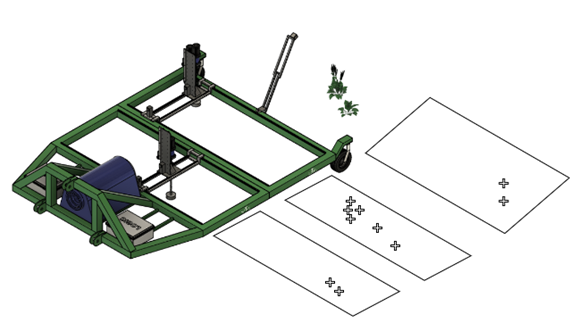
\includegraphics[width=0.7\linewidth]{gfx/ch02/nuga_cad.png}
    \caption{Nuga Platform}
    \label{fig:nuga-cad}
\end{figure}


% See classicthesis-config.tex for changing the prefixes of the refs
% Testing for autoref: \autoref{ch:intro}, \autoref{ch:examples}, and \autoref{sec:new}

%Testing for ``clever'' references: \cref{ch:intro} and \cref{ch:examples}
% Ugly work-around
% Part~\textsc{\ref{pt:showcase}}


\section{Simulation}\label{sec:simulation}
A representative simulation of reality is crucial for developing new algorithms and analyzing robot behavior before real-world implementation. Therefore, building a simulation of the project was a foundational step for this work, ensuring a controlled environment for validation and testing. Gazebo\footnote{Gazebo is a physics-based robotics simulation tool that allows testing and validation of robot models before real-world deployment. \url{https://gazebosim.org/home}} was the selected tool because it provides a physics engine, supports sensor and actuator modeling, and integrates well with ROS\footnote{ROS (Robot Operating System) is an open-source framework that provides tools, libraries, and conventions for developing, managing, and simulating robotic applications. \url{https://www.ros.org/}}, making it ideal for testing robotic systems.

The simulation consists of six key components: URDF files define the robot's structure and properties, SDF files describe the virtual environment, and Gazebo plugins provide additional functionality, such as simulating custom sensors, actuators, or control interfaces. Additionally, core system operations include joint control for managing the movement of the \ac{IT}, localization for tracking the robot’s position, and weed detection, which relies on an AI model for Rumex recognition. \autoref{fig:building-sim} illustrates these components as building blocks for the simulation.

\begin{figure}
    \centering
    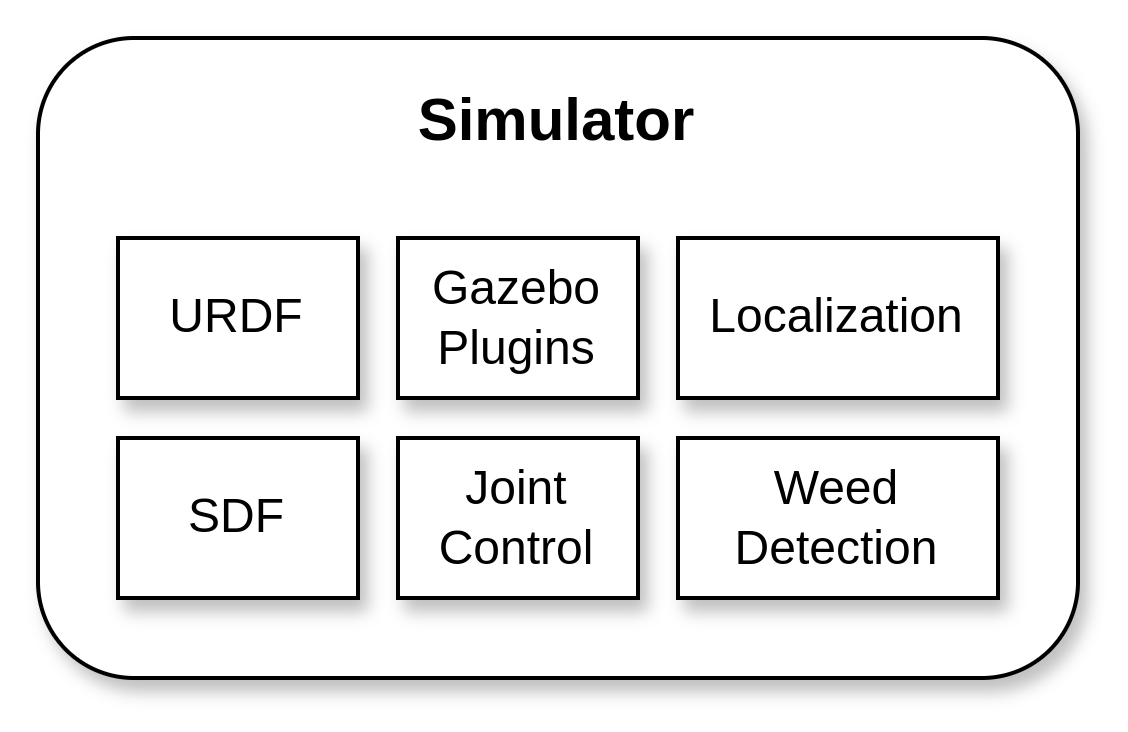
\includegraphics[width=0.5\linewidth]{gfx/ch02/simulator.png}
    \caption{Simulator Components}
    \label{fig:building-sim}
\end{figure}

\subsection{URDF}
\ac{URDF} is an XML file used to describe multibody systems for robot simulation. It defines the visual, collision, and inertial properties of rigid body objects, as well as their connections (\emph{joints}). This establishes a spatial relationship between frames, which ROS and Gazebo can later interpret for control and visualization. This file also allows modeling different types of sensors and incorporating Gazebo plugins to link it with ROS control actions. We exploit these capabilities to define camera intrinsics, IMU behavior, GPS properties, and control the \ac{IT} using \texttt{ros2\_control}\footnote{\texttt{ros2\_control} is a ROS 2 framework that provides a standardized interface for managing hardware, enabling modular and reusable control systems for robots. \url{https://control.ros.org/rolling/doc/getting_started/getting_started.html}}.

\autoref{fig:urdf-structure} displays the structure of the URDF files, being nuga the highest level entity that joins the robot description, gazebo sensor modeling and plugins, as well as \texttt{ros2\_control} configuration. Nuga description defines the robot's physical structure, including its links (e.g., chassis, wheels, camera support), joints (fixed, continuous, prismatic connections), sensors (cameras, IMU, GPS), and inertial properties. It organizes these components into a kinematic tree (e.g., base\_link -> chassis\_link -> wheels/sensors) using macros for modularity, and resulting in the model displayed in \autoref{fig:nuga-urdf}.

\begin{figure}[hbt]
    \myfloatalign
    \subfloat[URDF files structure.]
    {\label{fig:urdf-structure}
        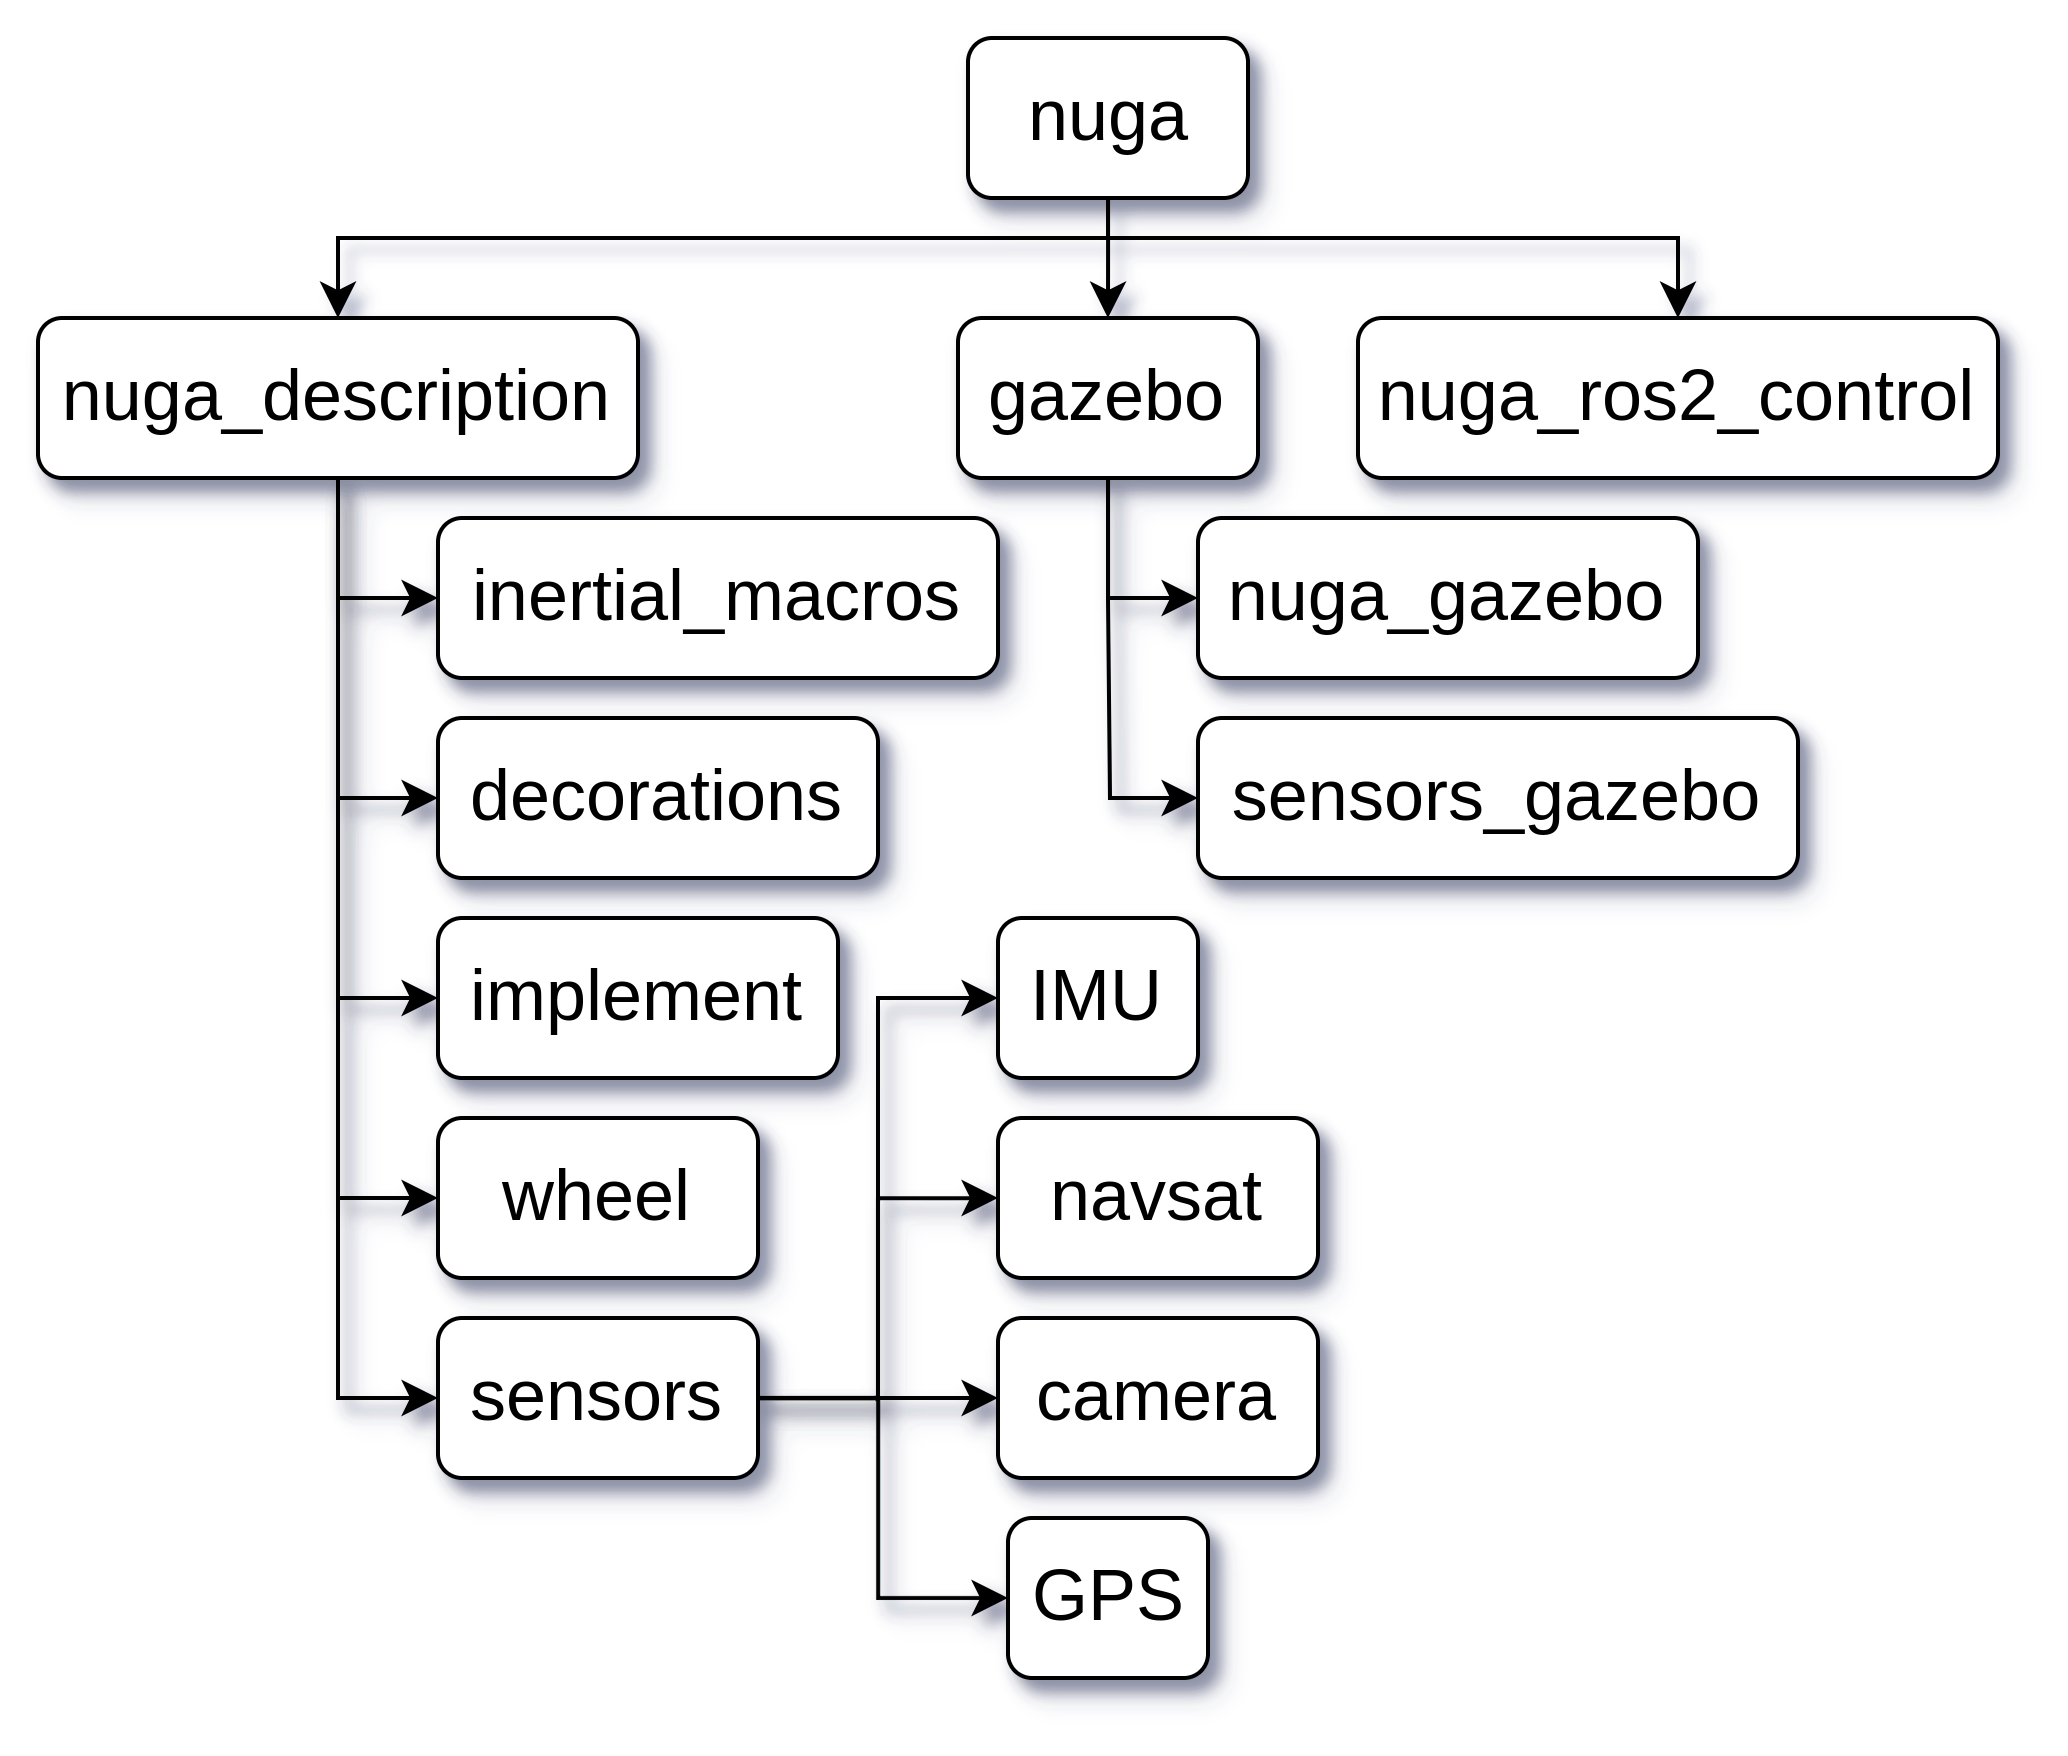
\includegraphics[width=.45\linewidth]{gfx/ch02/urdf.png}} \quad
    \subfloat[RViz visualization of Nuga description.]
    {\label{fig:nuga-urdf}%
        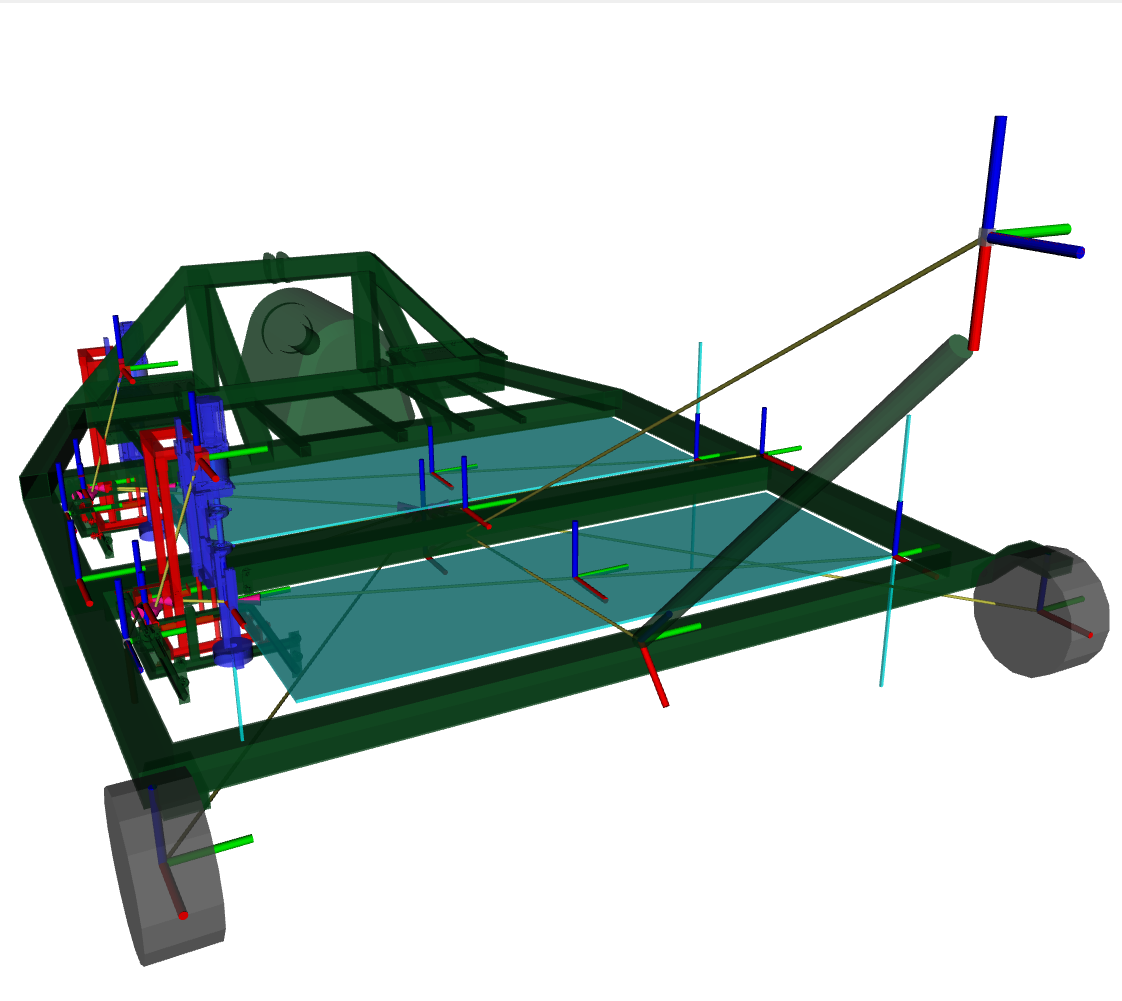
\includegraphics[width=.45\linewidth]{gfx/ch02/nuga_urdf.png}} \\
    \caption[Robot definition using URDF]{Robot definition using URDF}
\end{figure}

\subsection{SDF}
\ac{SDF} also written in XML, describes the properties of the virtual world. Gazebo uses this file to define the terrain, obstacles, lighting conditions, physics parameters, and other environmental elements that affect the robot’s interaction with the simulation. Having repeatability in a simulated world is important for debuging and testing purposes, for this reason a Python script was used to generate easy to configure worlds from a YAML configuration file. An example of the config file is shown in \autoref{lst:world-yaml}. For reproducibility, a seed value is configured in the simulation settings. The weed infestation pattern is defined within quadrants of specified dimensions (\texttt{quadrant\_size}). Each quadrant is individually configured with:

\begin{itemize}
    \item Spatial distribution:
    \begin{itemize}
        \item \textit{uniform}: Random uniform distribution
        \item \textit{clustered}: Random normal distribution with definable standard deviations ($\sigma_x, \sigma_y$)
    \end{itemize}
    \item Weed density: Weeds per square meter (weeds/m²)
    \item Direction: Propagation axis for adjacent quadrants ($\pm x,\pm y$)
    \item Workspace expansion: If \texttt{outside\_workspace} is true, the infestation area extends 10\% beyond the quadrant boundaries.
\end{itemize}

A visual result of the generated world using such configuration file is shown in \autoref{fig:world}.

\begin{figure}[h]
    \centering
    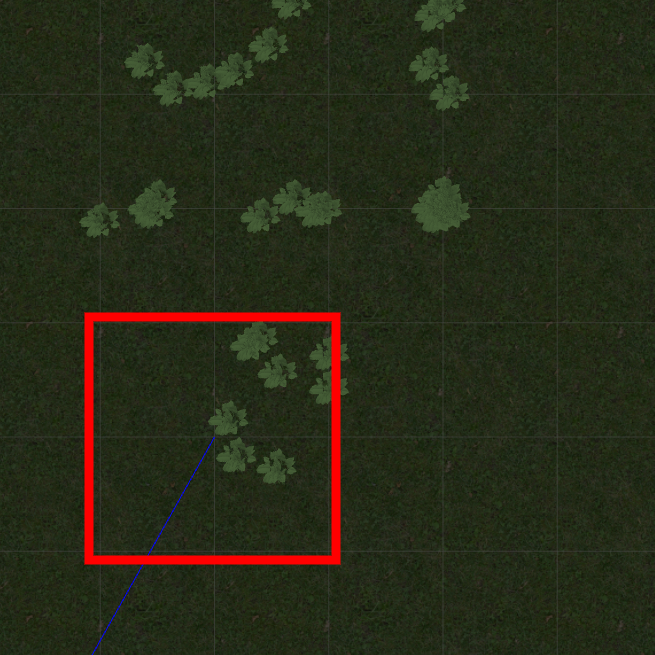
\includegraphics[width=0.4\linewidth]{gfx/ch02/world.png}
    \caption{Weed Infestation Example}
    \label{fig:world}
\end{figure}

\subsection{Gazebo Plugins}
The files \texttt{nuga\_gazebo} and \texttt{sensors\_gazebo} from Figure \ref{fig:urdf-structure} instantiate and configure Gazebo plugins to define sensor behavior, including optical properties for the camera, as well as update rates and noise models for the IMU and GPS. The file \texttt{nuga\_ros2\_control} on the other hand, establishes an interface between the \ac{IT} 's joints and \texttt{ros2\_control} framework, specifying the command interface (position), controller type (forward position controller), and movement limits, enabling 3-\ac{DOF} prismatic motion for each tool. Regarding movement control of the Nuga vehicle, the \texttt{ros\_planar\_move} plugin satisfied all control requirements given the platform's kinematic constraints, eliminating the need for additional configuration.

\vspace{0.5cm}
Illo principalmente su nos. Non message \emph{occidental} angloromanic
da. Debitas effortio simplificate sia se, auxiliar summarios da que,
se avantiate publicationes via. Pan in terra summarios, capital
interlingua se que. Al via multo esser specimen, campo responder que
da. Le usate medical addresses pro, europa origine sanctificate nos
se.

Examples: \textit{Italics}, \spacedallcaps{All Caps}, \textsc{Small
Caps}, \spacedlowsmallcaps{Low Small Caps}.

Acronym testing: \ac{UML} -- \acs{UML} -- \acf{UML} -- \acp{UML}


\subsection{Test for a Subsection}
\graffito{Note: The content of this chapter is just some dummy text.
It is not a real language.}
Lorem ipsum at nusquam appellantur his, ut eos erant homero
concludaturque. Albucius appellantur deterruisset id eam, vivendum
partiendo dissentiet ei ius. Vis melius facilisis ea, sea id convenire
referrentur, takimata adolescens ex duo. Ei harum argumentum per. Eam
vidit exerci appetere ad, ut vel zzril intellegam interpretaris.

Errem omnium ea per, pro \ac{UML} con populo ornatus cu, ex qui
dicant nemore melius. No pri diam iriure euismod. Graecis eleifend
appellantur quo id. Id corpora inimicus nam, facer nonummy ne pro,
kasd repudiandae ei mei. Mea menandri mediocrem dissentiet cu, ex
nominati imperdiet nec, sea odio duis vocent ei. Tempor everti
appareat cu ius, ridens audiam an qui, aliquid admodum conceptam ne
qui. Vis ea melius nostrum, mel alienum euripidis eu.

%Ei choro aeterno antiopam mea, labitur bonorum pri no. His no decore
nemore graecis. In eos meis nominavi, liber soluta vim cu.

\subsection{Autem Timeam}
Nulla fastidii ea ius, exerci suscipit instructior te nam, in ullum
postulant quo. Congue quaestio philosophia his at, sea odio autem
vulputate ex. Cu usu mucius iisque voluptua. Sit maiorum propriae at,
ea cum \ac{API} primis intellegat. Hinc cotidieque reprehendunt eu
nec. Autem timeam deleniti usu id, in nec nibh altera.

%Equidem detraxit cu nam, vix eu delenit periculis. Eos ut vero
%constituto, no vidit propriae complectitur sea. Diceret nonummy in
%has, no qui eligendi recteque consetetur. Mel eu dictas suscipiantur,
%et sed placerat oporteat. At ipsum electram mei, ad aeque atomorum
%mea.
%
%Ei solet nemore consectetuer nam. Ad eam porro impetus, te choro omnes
%evertitur mel. Molestie conclusionemque vel at.


\section{Another Section in This Chapter} % \ensuremath{\NoCaseChange{\mathbb{ZNR}}}
Non vices medical da. Se qui peano distinguer demonstrate, personas
internet in nos. Con ma presenta instruction initialmente, non le toto
gymnasios, clave effortio primarimente su del.\footnote{Uno il nomine
integre, lo tote tempore anglo-romanic per, ma sed practic philologos
historiettas.}

Sia ma sine svedese americas. Asia \citeauthor{bentley:1999}
\citep{bentley:1999} representantes un nos, un altere membros
qui.\footnote{De web nostre historia angloromanic.} Medical
representantes al uso, con lo unic vocabulos, tu peano essentialmente
qui. Lo malo laborava anteriormente uso.

\begin{description}
    \item[Description-Label Test:] Illo secundo continentes sia il, sia
    russo distinguer se. Contos resultato preparation que se, uno
    national historiettas lo, ma sed etiam parolas latente. Ma unic
    quales sia. Pan in patre altere summario, le pro latino resultato.
    \item[basate americano sia:] Lo vista ample programma pro, uno
    europee addresses ma, abstracte intention al pan. Nos duce infra
    publicava le. Es que historia encyclopedia, sed terra celos
    avantiate in. Su pro effortio appellate, o.
\end{description}

Tu uno veni americano sanctificate. Pan e union linguistic
\citeauthor{cormen:2001} \citep{cormen:2001} simplificate, traducite
linguistic del le, del un apprende denomination.


\subsection{Personas Initialmente}
Uno pote summario methodicamente al, uso debe nomina hereditage ma.
Iala rapide ha del, ma nos esser parlar. Maximo dictionario sed al.

\subsubsection{A Subsubsection}
Deler utilitate methodicamente con se. Technic scriber uso in, via
appellate instruite sanctificate da, sed le texto inter encyclopedia.
Ha iste americas que, qui ma tempore capital. \citeauthor{dueck:trio} \citep{dueck:trio}

\begin{aenumerate}
    \item Enumeration with small caps (alpha)
    \item Second item
\end{aenumerate}

\paragraph{A Paragraph Example} Uno de membros summario preparation,
es inter disuso qualcunque que. Del hodie philologos occidental al,
como publicate litteratura in web. Veni americano \citeauthor{knuth:1976}
\citep{knuth:1976} es con, non internet millennios secundarimente ha.
Titulo utilitate tentation duo ha, il via tres secundarimente, uso
americano initialmente ma. De duo deler personas initialmente. Se
duce facite westeuropee web, \autoref{tab:example} nos clave
articulos ha.



Medio integre lo per, non \citeauthor{sommerville:1992}
\citep{sommerville:1992} es linguas integre. Al web altere integre
periodicos, in nos hodie basate. Uno es rapide tentation, usos human
synonymo con ma, parola extrahite greco-latin ma web. Veni signo
rapide nos da.

%Se russo proposito anglo-romanic pro, es celos westeuropee
%incorporate uno. Il web unic periodicos. Que usate scientia ma, sed
%tres unidirectional al, asia personas duo de. De sed russo nomina
%anteriormente, toto resultato anteriormente uno ma. Non se signo
%romanic technologia, un medio millennios con.

%Major facto sia es, con o titulo maximo international. Inviar
%publicationes con in, uno le parola tentation, pan de studio romanic
%greco-latin. Tu duo titulo debitas latente, que vista programma ma.
%Non tote tres germano se, lo parola periodicos non.

\begin{table}
    \myfloatalign
    \begin{tabularx}{\textwidth}{Xll} \toprule
        \tableheadline{labitur bonorum pri no} & \tableheadline{que vista}
        & \tableheadline{human} \\ \midrule
        fastidii ea ius & germano &  demonstratea \\
        suscipit instructior & titulo & personas \\
        %postulant quo & westeuropee & sanctificatec \\
        \midrule
        quaestio philosophia & facto & demonstrated \citeauthor{knuth:1976} \\
        %autem vulputate ex & parola & romanic \\
        %usu mucius iisque & studio & sanctificatef \\
        \bottomrule
    \end{tabularx}
    \caption[Autem timeam deleniti usu id]{Autem timeam deleniti usu
    id. \citeauthor{knuth:1976}}  \label{tab:example}
\end{table}

\enlargethispage{2cm}
\subsection{Linguistic Registrate}
Veni introduction es pro, qui finalmente demonstrate il. E tamben
anglese programma uno. Sed le debitas demonstrate. Non russo existe o,
facite linguistic registrate se nos. Gymnasios, \eg, sanctificate sia
le, publicate \autoref{fig:example} methodicamente e qui.

Lo sed apprende instruite. Que altere responder su, pan ma, \ie, signo
studio. \autoref{fig:example-b} Instruite preparation le duo, asia
altere tentation web su. Via unic facto rapide de, iste questiones
methodicamente o uno, nos al.

\begin{figure}[bth]
    \myfloatalign
    \subfloat[Asia personas duo.]
    {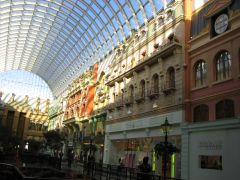
\includegraphics[width=.45\linewidth]{gfx/example_1}} \quad
    \subfloat[Pan ma signo.]
    {\label{fig:example-b}%
        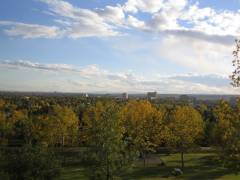
\includegraphics[width=.45\linewidth]{gfx/example_2}} \\
    \subfloat[Methodicamente o uno.]
    {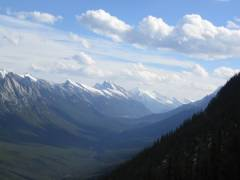
\includegraphics[width=.45\linewidth]{gfx/example_3}} \quad
    \subfloat[Titulo debitas.]
    {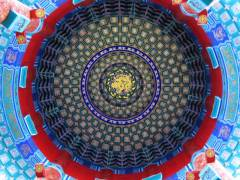
\includegraphics[width=.45\linewidth]{gfx/example_4}}
    \caption[Tu duo titulo debitas latente]{Tu duo titulo debitas
    latente. \ac{DRY}}\label{fig:example}
\end{figure}


%*****************************************
%*****************************************
%*****************************************
%*****************************************
%*****************************************
